% !TEX root = ../master-thesis.tex

\begin{figure}[h]
    \centering
    \addletter{85}{a}
    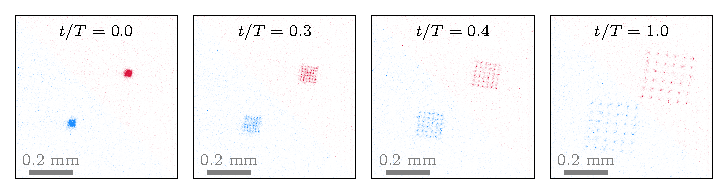
\includegraphics{fig-py/movement-inset.pdf} \\
    \addletter{115}{b}
    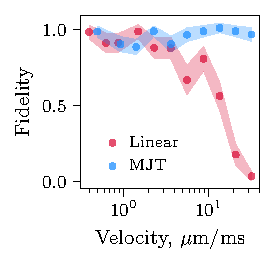
\includegraphics{fig-py/movement-1.pdf}
    \hspace{1cm}
    \addletter{115}{c}
    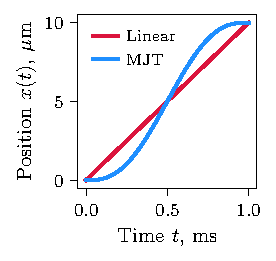
\includegraphics{fig-py/movement-2.pdf}
    \caption{
    \textbf{Characterization of tweezer transport protocols.}
    (a) Snapshots at different fractions of the total transport duration, illustrating atom movement between initial and target tweezer positions during a typical experimental run.
    (b) Comparison of transport fidelity as a function of velocity for the Minimum-Jerk Trajectory (MJT) and linear trajectory. Fidelity is defined as the probability of detecting an atom after transport, conditional on its initial presence.
    (c) Position versus time curves for MJT and linear transport trajectories.
    Data points correspond to measurements, shaded areas represent standard deviation across realizations.
    }
    \label{fig:movement}
\end{figure}